The NINJA-1 project was a huge success in bringing the numerical
relativity and gravitational-wave astronomy communities together, and
in providing intriguing qualitative results.  However, it only began
the process of testing detection and parameter estimation pipelines
against realistic signals.  The follow-up project, NINJA-2, is ongoing
as of the time of writing.  It's goal is to begin to quantify the
behaviors of pipelines in varying regions of signal parameter space
and suggest strategies for the advanced-LIGO era.


\section{Hybrid pN/NR waveforms}

\subsection{Verifying the hybrid waveforms}


\begin{figure}
  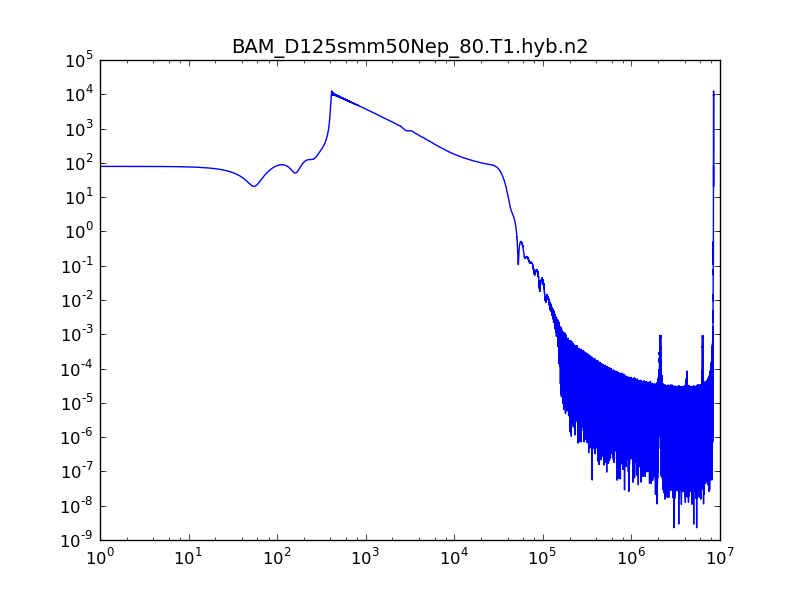
\includegraphics[width=0.5\linewidth]{figures/ninja2/bam_d125smm50nep_80_t1_hyb_n2_amp.png}
  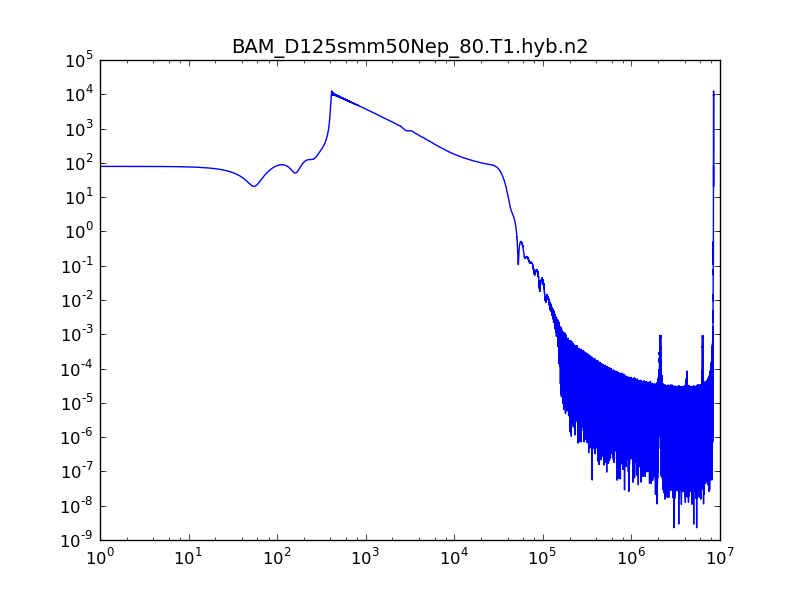
\includegraphics[width=0.5\linewidth]{figures/ninja2/bam_d125smm50nep_80_t1_hyb_n2_amp.png}
  \caption[Frequency-domain hybrid NINJA-2 waveforms]{
  \label{f:ninja2_freq_hybrids}
Fourier amplitude of the (2,2) mode of a sample NINJA-2
hybrid waveform from the BAM/AEI group.
\Note{I should remake these in scaled to $10\msun$ to give the axes
units}  The waveform on the left is the version initially submitted,
note there is a visible ``kink'' in the waveform at the hybridization
frequency.  The waveform on the right has been re-hybridized and there
is no longer a visible kink.  This feature did not show up in the time
domain view of the waveform.}
\end{figure}%

\begin{figure}
  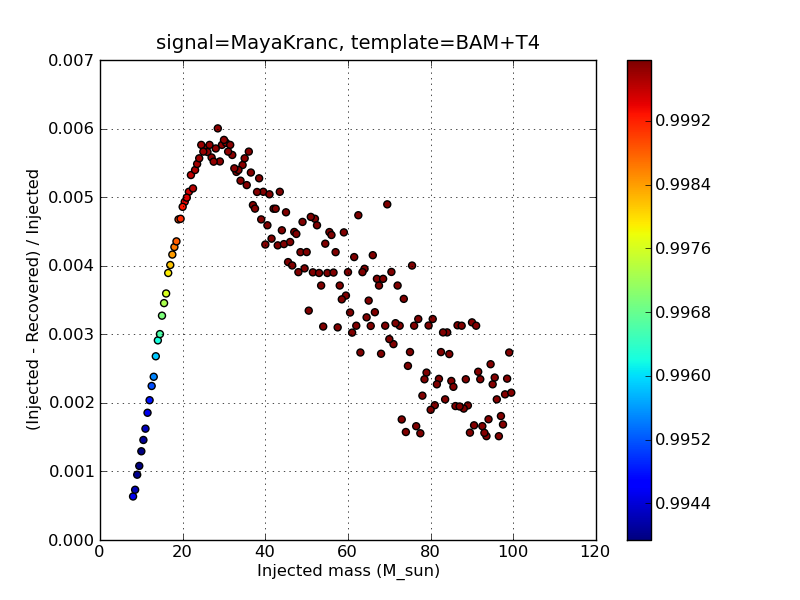
\includegraphics[width=0.5\linewidth]{figures/ninja2/maya_bamt4_max_over_m}
  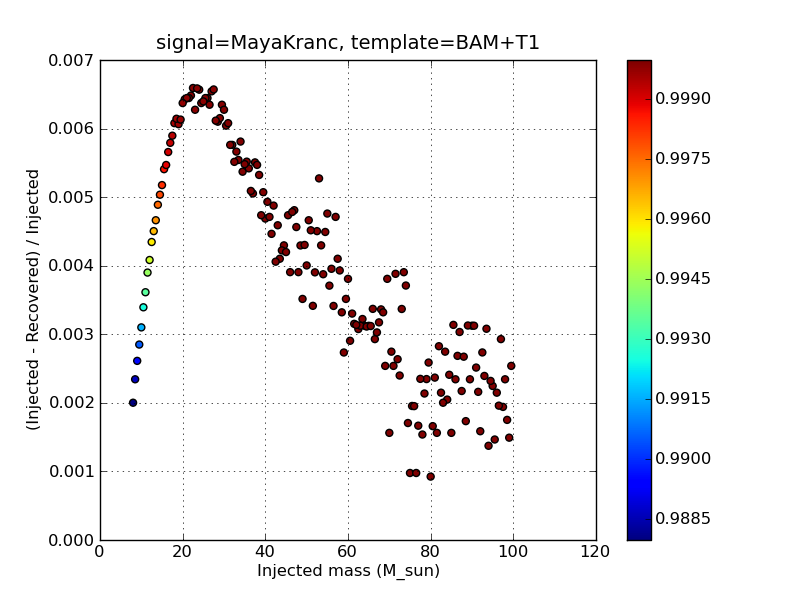
\includegraphics[width=0.5\linewidth]{figures/ninja2/maya_bamt1_max_over_m}
  \caption[Overlaps between NINJA-2 submissions maximized over mass]{
  \label{f:ninja2_max_over_mass_bam}
Overlaps between the equal-mass, non-spinning MayaKranc waveform taken
as the signal, and the equal-mass, non-spinning BAM waveform
hybridized with TaylorT4 (left) and TaylorT1 (right) taken as
templates.  Maximization is done over mass, as well as time and phase.
Note the lower overall overlaps and mass bias at the low-mass end,
where the two pN waveforms dominate the overlap.}
\end{figure}%


\section{Construction of the NINJA-2 data set}

\section{Data analysis}


%
\begin{table}
\begin{center}
\begin{tabular}{|l|l|}\hline
Group & Analysis \\\hline
Cardiff/Syracuse & Standard and extended CBC pipelines \\
GSTLAL & Matched filter, inspiral, merger and ringdown \\
 & spin-aligned templates \\
Urbino & Matched filter PhenSpinInspiralRD templates \\
UMass & Burst search with Omega pipeline \\
Washington State & CBC high-mass with coherent stage \\
Northwestern/MIT & Parameter estimation with LALInference \\
inspnest & Parameter estimation and model selection \\
 & with nested sampling \\
Ringdown & Matched filter, ringdown templates \\
AEI Hannover/UF Waveburst & Burst search with coherent Waveburst \\
UMD & CBC high-mass with EOBNRv2 templates \\
\hline
\end{tabular}
\end{center}
\caption[The data-analysis contributions to the NINJA-2 project.]{
\label{tab:ninja2-allda}
The data-analysis contributions to the NINJA-2 project.}
\end{table}

\subsection{preliminary results}


% TODO:
% make tables of submissions
% plot of paramater space in eta, chi scaled to 10 M
% plot of injection set (use chi instead of sum of magnitudes)
% text
% results

